% Implementation
\graphicspath{ {images/} }

This chapter discusses the platform and the programming techniques employed to
implement the application.  This is a web application meant to run
on desktop and mobile browsers. Traditionally, Javascript or programing languages which transpile
to Javascript are employed to execute such web apps. 

In the implementation of this application a functional programming language
called Elm which transpiles to Javascript is used. Therefore, the chapter
starts with explaining the benefits of using a functional programming in general
and introducing how Elm uses Model, View, Update architecture to implement a dynamic
front end.

I will discuss how a Graph as a
data-structure is defined and how it is drawn on screen as SVG (Scalable Vector
Graphics), how a function generates a colour palette for the colouring of the
vertices, how vertices are laid out in various geometrical patterns, and finally how
animations are implemented and graphs are made to change shape and translate in
2D space among other things.


\section{Front End Development with The Elm Programming Language}

The project is developed using the Functional Programming paradigm. This is a
paradigm which has been in development and practice since the days of infancy
of computer science. Functional programming is based on a form of computation
called lambda calculus proposed by Alonzo Church. \cite{Hudak2007}

For most of the history of computing, functional programming remained in the
ivory towers of academic research for purposes of exploring theoretical computer
science and language research.

In the last decades however, programming languages such as Haskell and a few
dialects of LISP have escaped the ivory towers to find application in the
software industry.

In this section I will discuss, why functional programming was chosen as the
programming paradigm of choice. How the functional programming language called
Elm is used to write a well structured, maintainable, intuitive and
understandable code to produce a dynamic front end.

\subsection{Why Functional Programming?}
Functional programming, makes the programmer think in a different way than the
may more popular imperative programming. In the functional paradigm, functions are
first class citizens, which can be mashed up together in myriad different ways
such as:


\begin{enumerate}
\item A function given as input to a another function,
\item A function producing another function as an output,
\item Composition of two functions dove-tailed to each other to produce another function,
\item Programming patterns being abstracted out as functions,
\end{enumerate}

For such Lego like usage of functions they must be dependable, such that for a
particular input a function will give a particular output just like
mathematical functions and has no business outside its scope for side-effects.
With such confidence in the functions, they can be fitted with each other to
make them do complex computation. \cite{Hughes89}

Since the functional paradigm is more reasonable and logical than imperative
programming the runtime errors are substantially less frequent than imperative
programming and is easier to maintain.


\subsubsection{Separation of Concerns}
If functions do not have side effects, how do they print
output on the terminal or read file from the hard disk or accept inputs from a
user? Functional programming environments have a way of separating the pure
part of a program from the impure part, by introducing `actions'. These
`actions' or side-effects are treated as a form of encapsulated data, which
can be manipulated by pure functions, and the environment makes changes to the
outside world by executing these actions.

Therefore the programmer has to write a large part of the program where he
deals with just pure functions. This allows them to exploit the perfectness of
pure functional programming.

This separation of concerns of pure and impure code in the context of the Elm
programming language is discussed in the \autoref{elm: architecture}
\emph{the Elm Architecture}.

\subsection{Why Elm Programming Language for This Project?}

For the reasons in the previous sections, a functional programming language was
chosen keeping in mind that the size of this project would be quite
substantial.  Unlike JavaScript, Elm does not require any external framework
such as Angular or React. This makes the program easier to reason with and
maintainable.

\subsubsection{Friendly Compiler Errors}
It has a compiler which gives developer friendly error messages almost guiding the
programmer for correct usage of the language. Refactoring code in Elm is easy
as the friendly compiler errors guide the programmer to each line of the code
which need modification while refactoring.

\subsubsection{Elm-Ui}
The layout of the application on the screen can be done without writing HTML and CSS by using an Elm library called Elm-Ui. This package frees the
programmer from using CSS styling and gives intuitive control of the page
layout with the help of rows and columns (Pure functions). With Elm-Ui,
multiple rows can be situated in a column and multiple columns can be situated
in a row. When elements are put in a row they are stacked side
by side horizontally. When the elements are put in a column they are stacked
one below each other. The elements in such a row or a column can be put at a
definite alignment and spacing from each other.

\begin{figure}[!ht]
\centering
\includegraphics[width=4.70in]{layout}
\caption{
         Implementation of the layout using the Elm-Ui library. The library helps implement a layout without having to write HTML and CSS. The page contains of two parent
         rows. The second row contains two columns, the left column contains
         the graphical display (SVG) part of the app, the second column is made up of
         rows containing explanation and buttons. The last row in the second column
         acts as the navigation bar to hop between the topics.
        }
\end{figure}

\subsubsection{Libraries and Community}
Elm also has rich libraries for linear algebra, graphics and Scalar Vector
Graphics which can aid in creating a \emph{2D} graphics web app like this one.
Elm also has a wonderful community help, advice and discussion on Slack and
Discord for example.

\subsection{The Elm Architecture}
\label{elm: architecture}
The Elm Architecture is a pattern of writing Elm code for responsive web
applications.  The architecture separates the concerns of front-end development
into:

\begin{enumerate}
\item Model,
\item View,
\item and Update.
\end{enumerate}

The Model is a data structure which holds the state of a program.
\cite{Fairbank19} This state is used by the view function as an input to
render the webpage.  The webpage, when rendered has elements, which may trigger
events, such as user inputs by the way of clicking an HTML element. Such events
are caught by the Elm runtime and sent to the update function.  The update
function takes these event messages and changes the state. The changed state is
then rendered by the view function to a modified page.  Therefore, the Model is
changed by the update function, then it is used by the view function to
render a webpage according to a formula set by the programmer. Hence the content
of the webpage reflects the state of the program.


\section{Events as Messages}
\label{impl: messages}
The events described in section \autoref{elm: architecture} generated by
animation clocks and clicks of the user on graph elements and buttons, are
called messages in Elm. For this particular
application they are defined as an Algebraic Data Type as:

\begin{lstlisting}[language=elm
                  , caption={
                              Abstract Data Type Msg with its Data Constructors.
                              These messages are dispached by buttons, graph vertices
                              system clocks and are received by the update function
                              to change the $Model$, which carries the state of the
                              program.
                  }
                  ]
type Msg
    = TimeDelta Float                  -- Clock Ticks for Animation
    | HoverOver Int                    -- Event when Mouse over a Vertex                              
    | MouseOut Int                     -- Event when Mouse out from a Vertex                               
    | VertexClicked Int                -- Event when Vertex Clicked                              
    | AnimationToggle                  -- Pause or Play Animation
    | AnimationStartOver               -- Restart Animation
    | ToggleVertexStatus Int           -- Select/Unselect Vertex
    | NextTopic                        -- Next Topic
    | PreviousTopic                    -- Previous Topic

\label{listing: Messages}
\end{lstlisting}

The messages are not just generated by user interaction with this application,
they are are also generated by the animation clock as can be seen in
the first data constructor of the type $Msg$.  The clock ticks and the key
strokes are events which initiate the update function to act on Model.  The
animation clock and key presses need to be subscribed from the Elm runtime in
the following way:

\begin{lstlisting}[language=elm
                  , caption={
                            Subscription of Animation clock and Key presses services.
                            Subscriptions are used to catch the events which are
                            emanated outside the DOM. In this code, a system clock
                            and key presses are subscribed to by the program.
                            }
                  ]
subscription : Model -> Sub Msg
subscription _ =
    Sub.batch
        [ E.onAnimationFrameDelta TimeDelta
        , E.onKeyPress keyDecoder
        ]
\label{listing: subsciption}
\end{lstlisting}

% Block diagram
\begin{figure}[h] % ’ht’ tells LaTeX to place the figure ’here’ or at the top of the page
\centering % centers the figure
\begin{tikzpicture}
% tikz code goes here
   \node[state] (q1) {Isomorphism};
   \node[state, right of=q1] (q2) {MaxkCut};
   \node[state, right of=q2] (q3) {Graphcoloring};
   \node[state, below of=q3] (q4) {VertexCover};
   \node[state, below of=q1] (q5) {TreeWidth};

   \draw (q1) edge[above, bend left] node{NextTopic} (q2)
         (q2) edge[below, bend left] node{PreviousTopic} (q1)
         (q2) edge[above, bend left] node{NextTopic} (q3)
         (q3) edge[below, bend left] node{PreviousTopic} (q2)
         (q3) edge[above, bend left] node{NextTopic} (q4)
         (q4) edge[below, bend left] node{PreviousTopic} (q3)
         (q4) edge[above, bend left] node{NextTopic} (q5)
         (q5) edge[below, bend left] node{PreviousTopic} (q4)
         (q5) edge[above, bend left] node{NextTopic} (q1)
         (q1) edge[below, bend left] node{PreviousTopic} (q5);
\end{tikzpicture}
\caption{This Finite State Machine (FSM) 
        shows how the messages, NextTopic and PreviousTopic
        changes the state of the program (the Model) from
        one topic to another. This is a subset of a much larger
        FSM in which the number of states and inputs are greater
        in number.
        }
\label{fig:my_label}
\end{figure}
% Block diagram
\section{Implementation of Graphs}
As part of the application state, a graph exists as data structure which contains a list of
vertices and a list of edges. The vertex, as can be seen in \autoref{code:
typeGraph} which is a data type defined separately consists of a name (which is
an integer), a colour, a 2D position (which had to be implemented using a 3D
vector, with z is always kept at zero).  An edge on the other hand is defined
as a combination of two vertices. Such Graphs are present in the Model in and
are used by the view function to be drawn as SVG.

\begin{lstlisting}[  language=elm, 
                     caption={
                              Definition of Vertex, Edge and Graph.  Vertex is
                              defined as a data structure which has a name as
                              an integer, a position as a 3 dimensional vector,
                              colour, and a flag which depicts if it has been
                              selected by the user.  An Edge has two Vertices and
                              a Graph contains a list of Vertices and a list of
                              Edges.
                             }
                  ,  label={code: typeGraph}
                  ]
-- Definition Vertex
type alias Vertex =
    { name : Int, pos : Vec3, color : color, glow : Bool }

-- Definition Edge
type alias Edge =
    { vertexOne : Vertex, vertexTwo : Vertex }

-- Definition Graph
type alias Graph =
    { vertices : List Vertex, edges : List Edge }
\end{lstlisting}

\subsection{Grid}
In the program a Grid is a list of 3D vectors or in other words a list of
position for vertices, which can be taken as an input by certain functions to
construct graphs or change shapes of graphs. 

A list of Vertices, for example can be formed by combining together lists of
names, colours and a grid.

Grids are important in implementing animations. In the animations a graph moves
towards a grid of positions. To aid this, there is a function, which which take
two grids and output a grid which is geometrically in between the two grids.
The graph changes from one intermediate grid to the next until it
reaches the final grid. This will be discussed in more depth in \autoref{animation:
morphing}.

\subsection{Using Linear algebra to Initialize Grids}
Linear algebra, in particular manipulation of vectors using Matrices has been
used to create interesting grids for the placement of vertices in the scene.
This includes rotation, scaling and translation of vectors to and from polygonal
patterns. Functions were created to form polygon with $n$ geometric vertices
which prove very handy in producing grids for various geometries like
the one seen in Graph Isomorphism and Max k Cut examples.

As a small example, here is a functional programming code in \autoref{code:
centroid} to find the centroid of three position vectors. You can observe
how first two vectors are added on line 3, and then it is pipelined to addition
with a third vector, which is in turn pipelined to being scaled by $0.33$
(divided by $3.0$). This could have been achieved in a single line of code, but
Elm reserves operators like $+$, $-$, $*$ for only numbers and they cannot be
overloaded to work for vectors.


\begin{lstlisting}[  language=elm
                  ,  caption={
                              Finding Centroid of Three Vertices. It logically
                              starts with vertex the addition of positions of
                              vertices $v_1$ and $v_2$. The output of which goes to
                              the same function at line 4 albeit partially
                              applied to position of $v_3$. The output, which is
                              the summation of the position of the three
                              vertices in turn is passed to a scale function
                              which effectively divides its input vector by
                              three. Hence the centroid emerges out of the
                              other end.
                             }
                  ,  label={code: centroid}
                  ]
findCentroidOfVertices : Vertex -> Vertex -> Vertex -> Vec3
findCentroidOfVertices v1 v2 v3 =
   Math.Vector3.add v1.pos v2.pos
   |> Math.Vector3.add v3.pos
   |> Math.Vector3.scale 0.333
\end{lstlisting}

\subsection{Creating Polygons}
Two dimensional graphics were used to create polygons to form the Grids
or subset of Grids for Graphs. Functional programming techniques such as mapping
over a list was employed to create and manipulate such grids. 
The construction of a polygon proceeds like this:

\begin{enumerate}
% Diagram is needed.
\item A list of floats containing ones is created. 

\item Each is converted to an angle in radians corresponding
to the polar position of the vertex. 

\item This list of angles is then presented to
a function which maps a horizontal vector with unit length over this list
such that the unit vector is rotated with an angle equal to the angle in the
list giving rise to a list of rotated vectors.

\item This regular polygon with vertices at unit distance from its center is
then scaled. The scaling factor for x is sometimes different from that of y.
Which enables squeezing of the polygon along any 2 dimensional direction.

\item Mixing such polygons come handy to create more complicated shapes.

\item The polygon is then translated to an appropriate position on the SVG screen.

\end{enumerate}

\subsection{Implementing colours}
To have a list of neighboring colours acting as a colour palette we work on the
Hue Saturation Lightness colour space (HSL), mostly varying the hue just pass a
region in the spectrum of hues (First, Second or Third) and the number of
colours needed as an Integer. On a scale from $0.00$ to $1.00$, the first region
will produce hues ranging from $0.00$ to $0.33$, the second producing it from
$0.33$ to $0.66$ and the third producing it between $0.66$ to $1.00$.

\subsection{Edges}
Edges are defined as a combination of two vertices. Since they are drawn as a
straight line segment between the positions of the two vertices, they do not require
positional data associated explicitly for them but are rather drawn out from the vertices
they contain.

\begin{figure}[!ht]
\centering
\includegraphics[width=4.22in]{Graph1New}
\caption{
         Drawing a Graph. Starting with a grid of positions
         a set of vertices are created. Connecting the vertices,
         the edges are formed according to a list of tuples. The 
         vertices is then laid on top of the edges by concatenating list
         of SVG elements representing edges with list of SVG elements
         of Vertices. This is followed by this new list being concatenated
         with a list of SVG text representing the vertex names.
        }
\end{figure}

\section{Implementation of Animations}
In this section I will cover how various animations in the
application are implemented. Though there are minor differences between animations
for one topic to another, they follow a common pattern. The common pattern is
this that events are generated by a quasi-regular clock. These events trigger
the update function which transforms the current state of the program and
changes the position of certain abstract entities. The view function while
redrawing these entities takes the position information from the updated model
to draw them as SVG.

\subsection{Morphing Geometry of a Graph}
\label{animation: morphing}
In some of the animations in the application, the graph changes its geometry
to visually look different than the original. This is accomplished by a
function which takes a graph and a grid to move the input graph incrementally
towards the grid with every tick of the animation clock.  When the animation is
started, with each tick of the animation clock, the vertices of the second
graph move towards the target grid points with a constant velocity.  The
velocity of a vertex is calculated by obtaining the displacement vector between
the target position and the current position of the vertex and also the time
available before the animation ends.  The displacement is calculated as
$\vec{d} = \vec{p_t} - \vec{p_v}$, where $\vec{p_t}$ is the target postion and
$\vec{p_v}$ is the current position of the vertex. The time available is
calculated as $t = t_{available} - t_{elapsed}$. The velocity is calculated as
$\vec{v} = \vec{d}/t$.  The distance the vertex must travel is hence calculated
as $\Delta d = \vec{v} \times \Delta t$.  Where $\Delta t$ is the time elapsed
since the last tick of the animation clock.


%PICTURE of Isomorphic Animation
\begin{figure}[h]
\centering
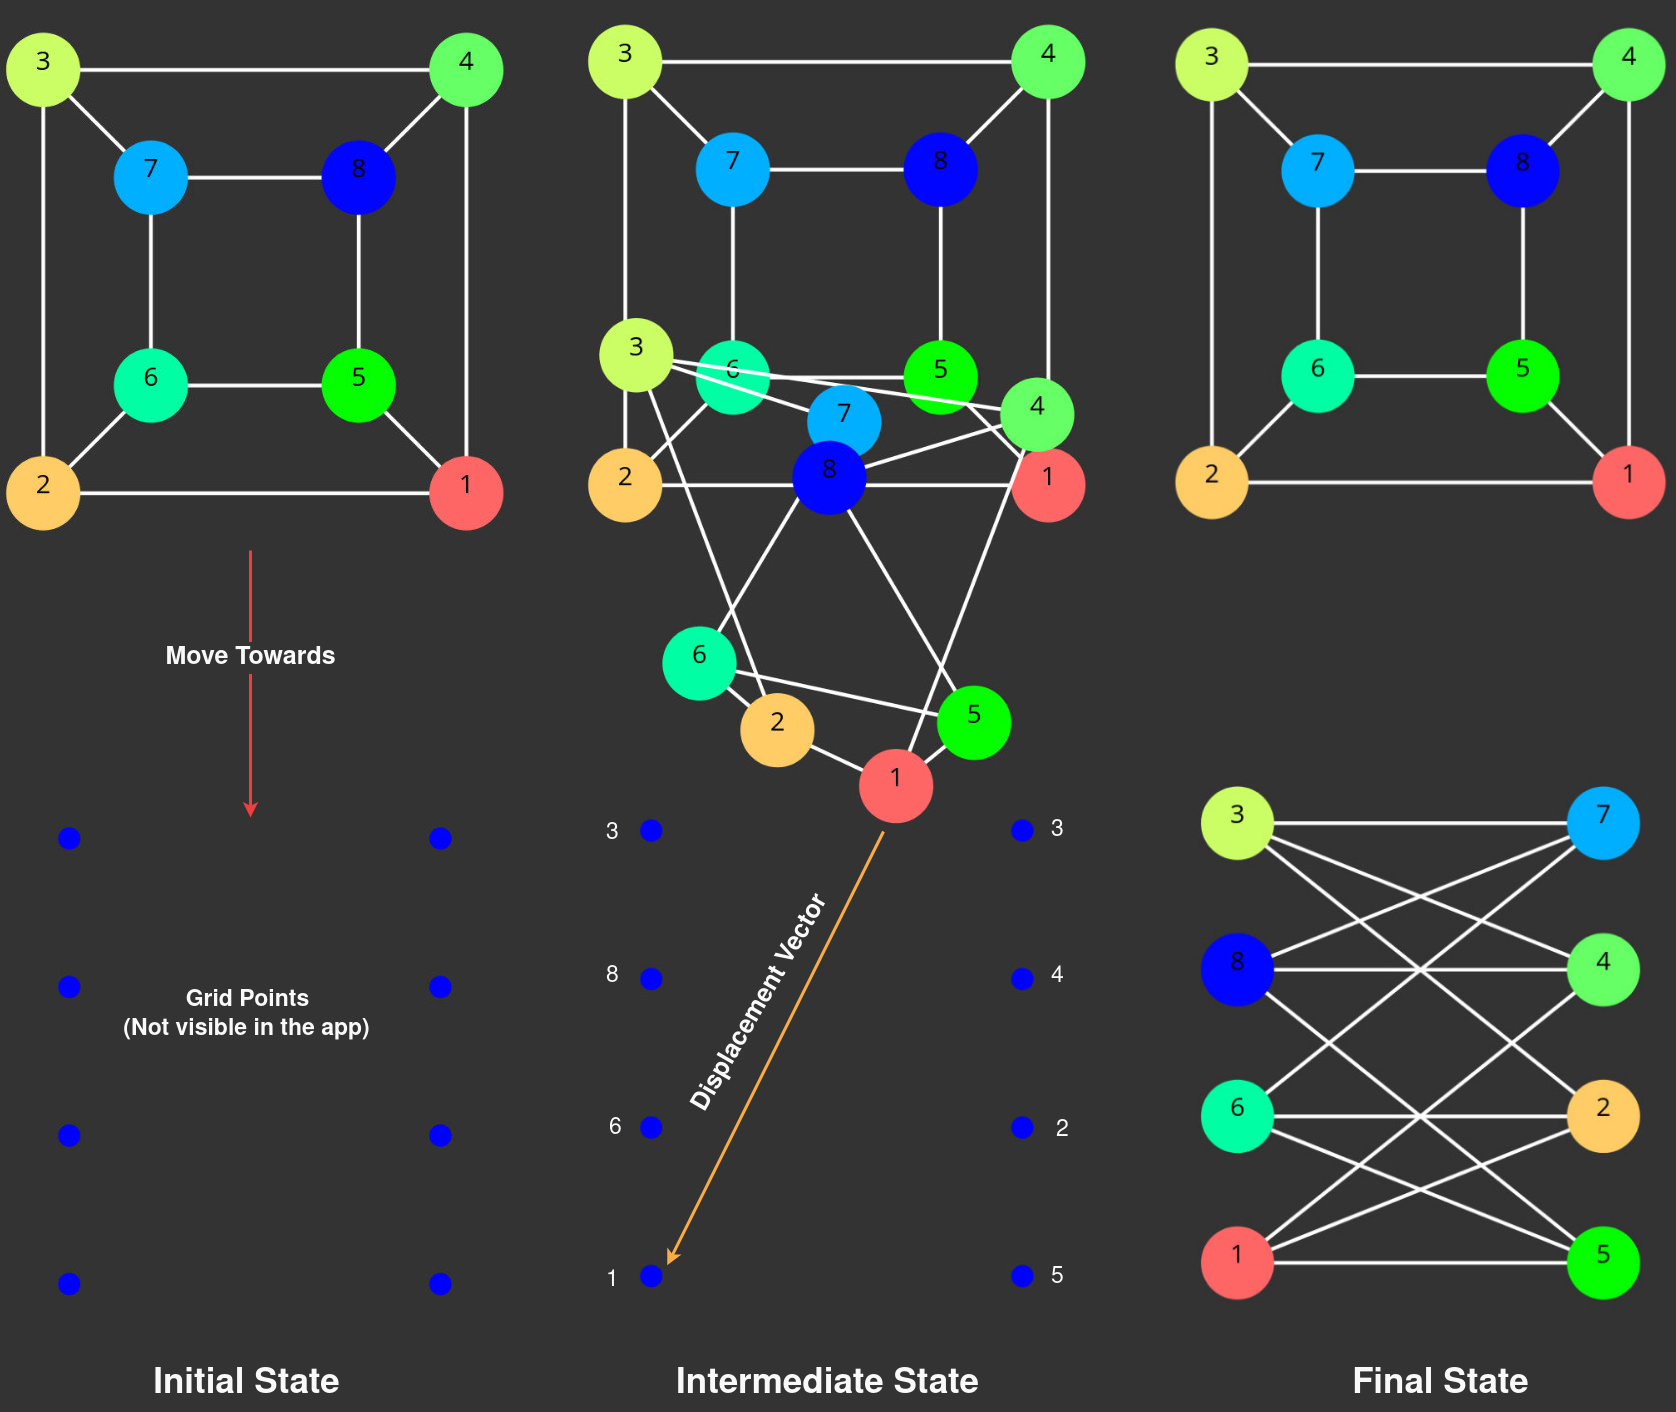
\includegraphics[width=4in]{IsomorphismAnimation}
\caption{
        Morphing a graph. This example from the Graph Isomorphism topic
        shows how shape transformation is done with the help of a targed grid.
        The target grid is shown as blue points. In the picture in the middle,
        a diplacement vector is shown between the current position of vertex 1
        and its final position. Veloicty of this vertex is calculated by deviding
        the displacement vector with the available time left in the animation.
        }
\label{animationfigure: isomorphism}
\end{figure}

\subsection{Re-formation of the Graphs}
At each tick of the animation clock the graph under transformation, is built
again, with vertices having the same name and colour as the original but new
positions. The edges need to be re-constructed again as the vertex positions
have been renewed. This is something which is expected in the functional
programming paradigm where nothing is changed in place and new data structures
are created with application of a function. This is true not just for
animations, it is true for user-interaction or anything which requires visual
(Geometric or colour) modification of the graph.

The re-formation of the vertices and the edges are shown in
the Elm function in \autoref{code: morphGraph}. The function takes a
graph and a grid and produces a new graph situated at the new grid with new
vertices and edges. The edges formed in the new graph are connected to the
same vertices (vertices with the same names) as the original ones.

\begin{lstlisting}[language=elm, 
      caption={
      Changing the shape of a graph for animation.
      The first line in the code excerpt describes the Type Signature of the function
      morphGraph. It says that the function takes a Graph and a Grid as input
      and produces a Graph as an output.
      The input Graph's vertices adopt the positions listed in the Grid.
   }
   , label={code: morphGraph}
   ]
morphGraph : Graph -> Grid -> Graph
morphGraph graph grid =
    let
        updatedVertices =
            List.map2 updatePositionVertex graph.vertices grid

        createEdge =
            updateEdge updatedVertices

        updatedEdges =
            List.map createEdge graph.edges
    in
    Graph updatedVertices updatedEdges

\end{lstlisting}

% Block diagram
\begin{figure}[ht] % ’ht’ tells LaTeX to place the figure ’here’ or at the top of the page
\centering % centers the figure
\begin{tikzpicture}
% tikz code goes here
   \node[state] (q1) {Initial Grid};
   \node[state, right of=q1] (q2) {Second Grid};
   \node[state, right of=q2, initial] (q3) {Penultimate Grid};
   \node[state, right of=q3] (q4) {Final Grid};

   \draw (q1) edge[above] node{TimeDelta} (q2)
         (q2) edge[draw=none] node{$\cdots$} (q3)
         (q2) edge[draw=none, above] node{TimeDelta(s)} (q3)
         (q3) edge[above] node{TimeDelta} (q4);
\end{tikzpicture}
\caption{ A Finite State Machine shows how the animation progresses with
          each tick of the elm run-time clock, depicted as the message TimeDelta.
          With each such message each vertex takes their
          respective position in the following grid.
        }
\label{fig: animationFSM}
\end{figure}
\subsection{Drawing of Graphs}
Drawing graphs is done using SVG elements. The vertices are drawn as colour
filled circles while the edges are drawn as straight line segments between the
positions of the related vertices. The edges are drawn first and the vertices
later so that vertices appear on top of the edges and the edges seem to be
appearing out of the surface of the vertices.

\section{Explanation Panel}

The Explanation Panel is always shown on the right and it consists of the title of the topic and suggestions on how
to interpret and interact with the animations.

The content of this panel depends on the state of the animation or the user
interaction associated with the topic.

The functions which populate the explanation panel with different elements have
therefore a subset of the \emph{Model} data structure as its input.  According
to the state of the program relevant advice, instructions and buttons are
shown on the panel.

The functions responsible for Explanation Panel in the case of user interaction
such as the ones in Graph colouring and minimum vertex cover run a check on the
state of the program to know if the user is doing their task correctly. For
example in graph colouring, if two adjacent vertices are coloured the same colour,
a warning message appears in the explanation panel.


\section{Navigation and Control}
There are several buttons and keyboard shortcuts to go from one topic to the
next and to play/pause and restart animations. These have been implemented by
generating appropriate messages which are caught by the update function which
in turn updates the model (state of the program). The updated model of the
program is reflected on the screen by the view function.

\subsection{Home Page}
See the design of home page in \autoref{design: home}.  The topic icons contain
miniaturized version of the graphs for the corresponding topics. The
miniaturized versions of the graph are borrowed from the implementation of the
various animations and user interactive tasks in the app.  The miniaturization
is implemented by spawning the SVGs in small spaces . As the graphics is
scalable, it adopts the size of its parent element.  Clicking on the Graph
Isomorphism icon, for example, triggers the $GoToIsomorphism$ message which is
used by the $update$ function to change the state of the model to contain the
$Isomorphism$ topic.


\subsection{URL Management}
Although there is only one HTML page rendered (this application being a Single
Page Application), when the user navigates from one topic to another they can see
the URL path after the Website's name change to reflect the pseudo-page he is
on. This change in the URL is brought by the function $pushUrl$ at appropriate
situations.  The change in the URL is detected by the run-time to produce the
message $UrlChanged$ which in turn is caught by the Update function to
re-populate the page with new topic.

\subsection{Navigation Bar}
The navigation bar consists of buttons to go to the previous and the next
topics.  When the message $PreviousTopic$ or the message $NextTopic$ is
generated by the buttons respectively, the update function catches it to change
the state of the program to load it with the
details of the previous/next topic.

\subsection{Keyboard Shortcuts}
Keyboard shortcuts provided a fast way to test various functionalities while
developing the application.  These functionalities have not been taken away
even after development therefore they still can be used to trigger events in
the application without the use of a pointer device. 
The key presses messages are registered by the elm run-time which in turn
triggers the update function to update the model. Information about the keyboard shortcuts can be
availed on the screen by pressing the information icon present in the
navigation bar. Below is an example list of a few key-bindings.

\begin{itemize}
\item \textbf{p}: Toggle between pause and play animation. (Can be used instead of the Play/Pause button; Generates the $AnimationToggle$ message). \\
\item \textbf{r}: Restart animation. (Can be used instead of Restart Button; Generates the $AnimationStartOver$ message). \\
\item \textbf{n}: Go to the next topic. (Can be used instead of the navigation button; Generates the $NextTopic$ message). \\
\item \textbf{N}: Go to the previous topic. (Can be used instead of the navigation button; Generates the $PreviousTopic$ message). \\
\item \textbf{t}: Next animation (Can be used in case of Max k Cut and Tree width to go to the next animation; Generates the $NextAnimation$ message)
\end{itemize}


\subsection{Screen Compatibility}
So that the various visual sections of the application occupy their appropriate
place on screens of different sizes, such as screens of of various laptops and
smart phones, the width and height of the screen is used to give the height and
width to each section.  
The state of the program stores data of the type $DeviceType$, which makes the
program aware of the screen size of the device being used. This data is used to
give proper font size to various text elements used in the app. Such measures,
have made the application friendly to mobile devices and changes in the browser
window size caused by the user on a personal computer.

\section{Implementation of Topics}
The above sections have discussed the basic building blocks which can be used
to implement the individual topics. The building blocks include graphs, animations
page-layout, navigation and control.

\subsection{Graph Isomorphism}
\label{impl: isomporphism}

This topic is elucidated by a user interactive animation and an animated quiz, discussed in detail in \autoref{story: isomorphism}. 


\subsubsection{Isomorphic Definition Animation}
The first animation consists of two Graphs which are the same.  In the
beginning the two graphs are superimposed with each other.  Each
graph is constructed by merging two polygons and connecting their vertices in a
wheel like structure. As the animation begins one graph leaves its position
and transforms to another shape.  This is achieved by instantiating the two
graphs with same position and form. An empty grid is also provided as the
target set of positions for the vertices of the second graph. 

When the user presses the play button the message $AnimationToggle$ is
generated. When the update function receives this message, it checks for the
state of the program which is set at $IsomorphicTransition$. It starts the
animation if it is not already in progress.  

When the animation is started, with each tick of the animation clock, the
vertices of the second graph move towards the target grid points with a
constant velocity. For the kinematics involved in this transition see
\emph{Morphing Geometry of a Graph} in \autoref{animation: morphing}.

%PICTURE of Isomorphic Quiz
\begin{figure}[h]
\centering
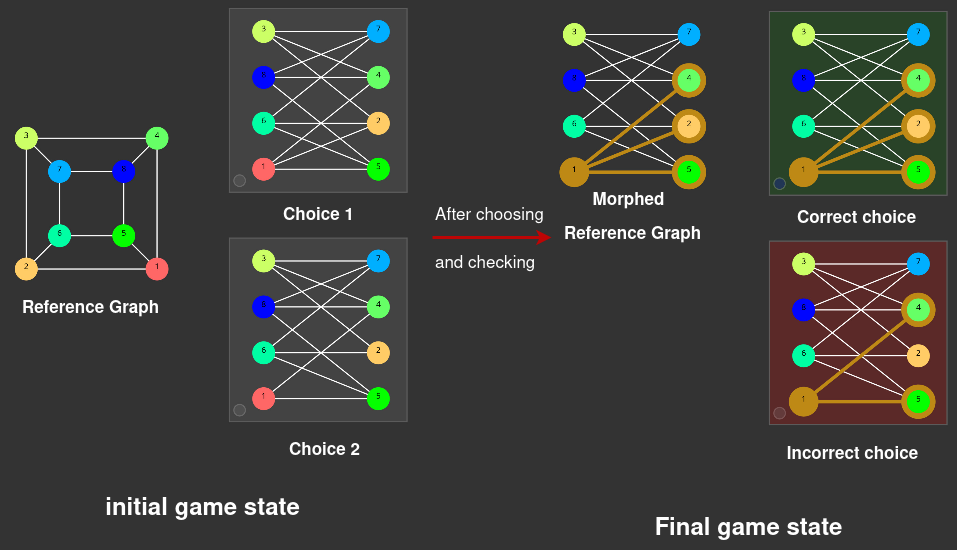
\includegraphics[width=4in]{isogame}
\caption{
         Graph Isomorphism Quiz. 
         \textbf{Left:} The user is presented with a reference graph on the left and two
         options on the right and asked which one of the two options are
         isomorphic to the reference one.
         \textbf{Right:} When the user makes his choice and checks the answer,
         then the right answer is shown in green background and the wrong in a red background.
         The edges which are essential in figuring which graphs are isomorphic to one-another
         are displayed differently in golden colour.
        }
\label{animationfigure: isomorphicGame}
\end{figure}
The animation is also user interactive: when the user hovers over a vertex, or
selects it by pressing the corresponding numerical key on the keyboard, a
Boolean variable associated with the vertex is turned \emph{True}. A function
filters the list of vertices to find the selected vertex. Another function
finds the edges incident on the vertex and also the vertices adjacent to the
selected vertex by filtering over the list of edges in the graph. These are
shown differently in a highlighted colour in both the graphs in the display
section.  The explanation section also uses this data to explain how the
selected vertex is connected to the same adjacent vertices in both the graphs.

\subsubsection{Animated Quiz for Graph Isomorphism}
The second activity gives the user three graphs. The first graph is a reference
graph. The user is asked to choose which one out of the two remaining graphs is
isomorphic to the reference graph. The right answer is hard coded, and when the
user selects his answer, the program checks if the answer chosen is right one
and changes the appearance of the display and the explanation panel.  The
state of the game consists of two variables: $Choice$ and $CheckState$.  When
the user has not made any choice yet $Choice$ is at $NoChoice$ state.  When the
choice is made, $Choice$ is set to $FirstGraph$ or the $SecondGraph$.  When the
user presses the button to check the answer $CheckState$ transforms from
$NoCheck$ to the $Check$ state.  There are case statements in the code which
take the correct measure depending on the state of the game.

\subsection{Max k Cut}
\label{impl: maxkcut}
The Max k Cut topic has two animations related to Max
2 Cut and then Max 3 Cut . See \autoref{story: maxkcut} for explanation of the
animations. The first animation has a graph constructed by merging two polygons.
The edges are defined so that the graph is nearly bipartite (see
\autoref{graphtheory: definitions} ) save for one edge (see \autoref{story:
max2cut}). The target grid for the animation is made of the combination of the
same polygons but set apart vertically. The kinematics of the animation is
executed the same way as is done for Graph Isomorphism.

The user can draw a predetermined line segment which separates the two
sets. The line segment is superimposed by intersection points of the
line segments and the edges between the two sets. An intersection point
is calculated by finding intersection of two line segments. A linear algebra
library function was used for this task.

%%PICTURE of Max  2 Cut Animation
%\begin{figure}[h]
%\centering
%\includegraphics[width=3.50in]{max2cutAnimation}
%\caption{
%        Arrangement of animation of Max 2 Cut.
%        }
%\label{animationfigure: max2cut}
%\end{figure}

%PICTURE of Max  3 Cut Animation
\begin{figure}[h]
\centering
\includegraphics[width=4.22in]{max3cutanimation}
\caption{
        Arrangement of animation of Max 3 Cut. This animation transforms a graph
        into a shape such that the three sets of vertices of the graph making a Max 3 cut
        are separated from each other distinctively. The three sets move away from each
        other in directions which are $120^{\circ}$ apart.
        }
\label{animationfigure: max3cut}
\end{figure}
In the case of Max 3 Cut (see \autoref{story: max3cut}), the animation begins
with a tripartite graph. The graph is based upon a regular \emph{nonagon}
shaped grid. The destination grid, in this animation is shape of an equilateral
triangle, with the grid points near the vertices of the said triangle. The
graph consists of three sets of vertices which settle down at the vicinity of
the three vertices of the equilateral triangle at the end of the animation. The
kinematics of the motion of the vertices is explained in \autoref{animation:
morphing}.

\subsection{Graph colouring}
This section has two user interactive tasks to colour graphs in the way they
should be coloured for a graph colouring problem.
The graph in the first task is composed of two concentric square graphs such
that each vertex has three adjacent vertices. The user task is to colour the
graph using two different colours. See \autoref{story: coloring} for further
explanation of the task.

The graph in the second task is composed of two concentric pentagonal graphs such
that each vertex has three adjacent vertices. The user task is to colour the
graph using three different colours. See \autoref{story: coloring} for further
explanation of the task.

When the user chooses a colour from the colour palette, the chosen colour is
updated in the state of the program. When the user clicks a vertex, the colour
of the vertex is changed with the colour stored in the state of the program.

%PICTURE of Graph colouring task
\begin{figure}[h]
\centering
\includegraphics[width=4.22in]{Graphcoloring}
\caption{
        Graph colouring Task. The graph on the left has a pair of incorrectly
        coloured vertices. On the right there is a fully and correctly coloured
        graph, where all the adjacent vertices are coloured differently from each
        other.
        }
\label{animationfigure: max3cut}
\end{figure}

A function performs checks while the user is working on the task, whether
two adjacent vertices have similar colour by doing a linear search on the edges.
If they are, the information is used to display a warning to mark that edge differently
and a warning appears on the explanation panel based on this search.

If in a linear search for finding adjacent vertices of the same colours
does not have an output and if all the vertices have been coloured, then
the function which populates text on the explanation panel shows a message that
the task is complete.

\subsection{Vertex Cover}


The user interaction for this topic asks the user to choose the minimum number
of vertices such that all the edges in the Graph belong to the set of vertices
which are incident on the chosen vertices, as detailed in \autoref{story: vertexcover}.

The user is given two tasks similar in nature. In the first task the graph in
the Vertex Cover is based on composition of two square grids. In the second
task the graph is based on composition of two hexagonal grids.  When the user
clicks on a Vertex, there is a Boolean value associated with the Vertex which
becomes \emph{True}. There is a function which filters the list of edges to
find which of them have at least one of their vertices \emph{selected}. Such
edges are illuminated, for the user to note that the edge has been covered.

%PICTURE of Vertex Cover task
\begin{figure}[ht]
\centering
\includegraphics[width=4.22in]{VertexCover}
\caption{
        Vertex Cover task. The graph on the left shows the selected vertex 5
        and the edges incident on it in golden colour. A vertex can be selected
        by either clicking the vertex or pressing the corresponding number key
        on the keyboard. The edges shown in golden colour are the ones which are
        covered, they are coloured so automatically when a vertex related to
        them is selected. The graph on the right has all its edges covered.
        }
\label{animationfigure: vertexCover}
\end{figure}

There is a function which filters out the edges whose one of the vertices
have been selected, and another which counts the number of vertices which
have been selected.  When the all the edges have been covered, the program
checks for the number of vertices selected to do this by filtering the list of
vertices. In the case of the particular example in this project, the graph can
be covered using four vertices. Therefore if the number of vertices selected at
the end of the session are greater than four, then the explanation panel is
populated with a message that the task needs to be attempted again. Finally, next task button loads the program with the new task.

\subsection{Tree Width}
Tree width topic is implemented in a series of animations.  In the first
animation the vertices of the graph of this topic are arranged circularly
albeit with edges such that there is a cellular structure in present inherently
in the graph. This edges were set up in this graph by coding their connectivity
in a list of tuples.
This is also a graph-transition just like graph isomorphism. The target grid
for this transition is a regular lattice which reveals the cellular nature of
the graph. The kinematics of the transition is the same as that of graph
isomorphism (see \autoref{impl: isomporphism}) and Max k Cut (see
\autoref{impl: maxkcut}). For more information on the kinematics of such shape
transitions see \autoref{animation: morphing}.

%PICTURE of Tree Width Animation
\begin{figure}[ht]
\centering
\includegraphics[width=4.22in]{TreeWidth}
\caption{
        Tree width Animations. From the top left to bottom left. Tree width is
        explained in a series of animations. The first animation turns the
        original graph to a cellular like structure by moving towards a
        pre-determined grid.  After the transformation a piece is defined as a
        subset of a graph.  The next graph shows how graph can be decomposed
        into several such pieces.  The last picture shows how the pieces can be
        connected together by a tree.
        }
\label{animationfigure: vertexCover}
\end{figure}

The second part of the animation highlights one piece of the cellular structure
. The piece is also marked by drawing a blue dot at the center
of it. The position of the blue dot is found by taking the centroid of the
constituent vertices of the piece.

In the third part the centroid of all the pieces are found and marked as blue.
These blue dots are connected by special lines in the last part of the
animation to form the tree structure inherent in the original graph. The animation series is followed step by step by explanation panel which responds
to the various stages of the user progressing through the task.


\section{Modules}

The program is divided into ten modules.  $Main$ holds a key role and acts as the launching pad for the program. It also serves as a connector, loading the features of specific graph theory topics as needed when navigation commands are issued.

The five topics included in the project own a module of their own. They are
$Isomorphism$, $Maxkcut$, $Graphcoloring$, $VertexCover$ and $TreeWidth$ modules.
These modules are imported by the main function to be used on the screen.
Henceforth these will be collectively known as the \emph{Topic Modules}.

Within the $Graph$ module there are data types and functions for representing,
constructing, drawing and animating the graphs. This module contains most of the
code related to geometry. This module is depended on by all the \emph{topic modules}.

The $Explanation$ module contains the text data as a $0-nary$ functions
(functions which do not take input) used by topic modules for the explanation of
the respective topics. These only contain the definitions of the concerned
graph theory problems.

Finally, the $Messages$ module contains the messages which are generated with system
clock ticks or user interaction with the DOM elements.  Such messages are
defined as \emph{Algebraical Data Types} (see \autoref{impl: messages}) and are
imported by almost all other modules. This along with the $Main$ and $Graph$
modules form the central pillar of the program and are the minimum requirement
of the program to function.

%PICTURE of modules
\begin{figure}[h]
\centering
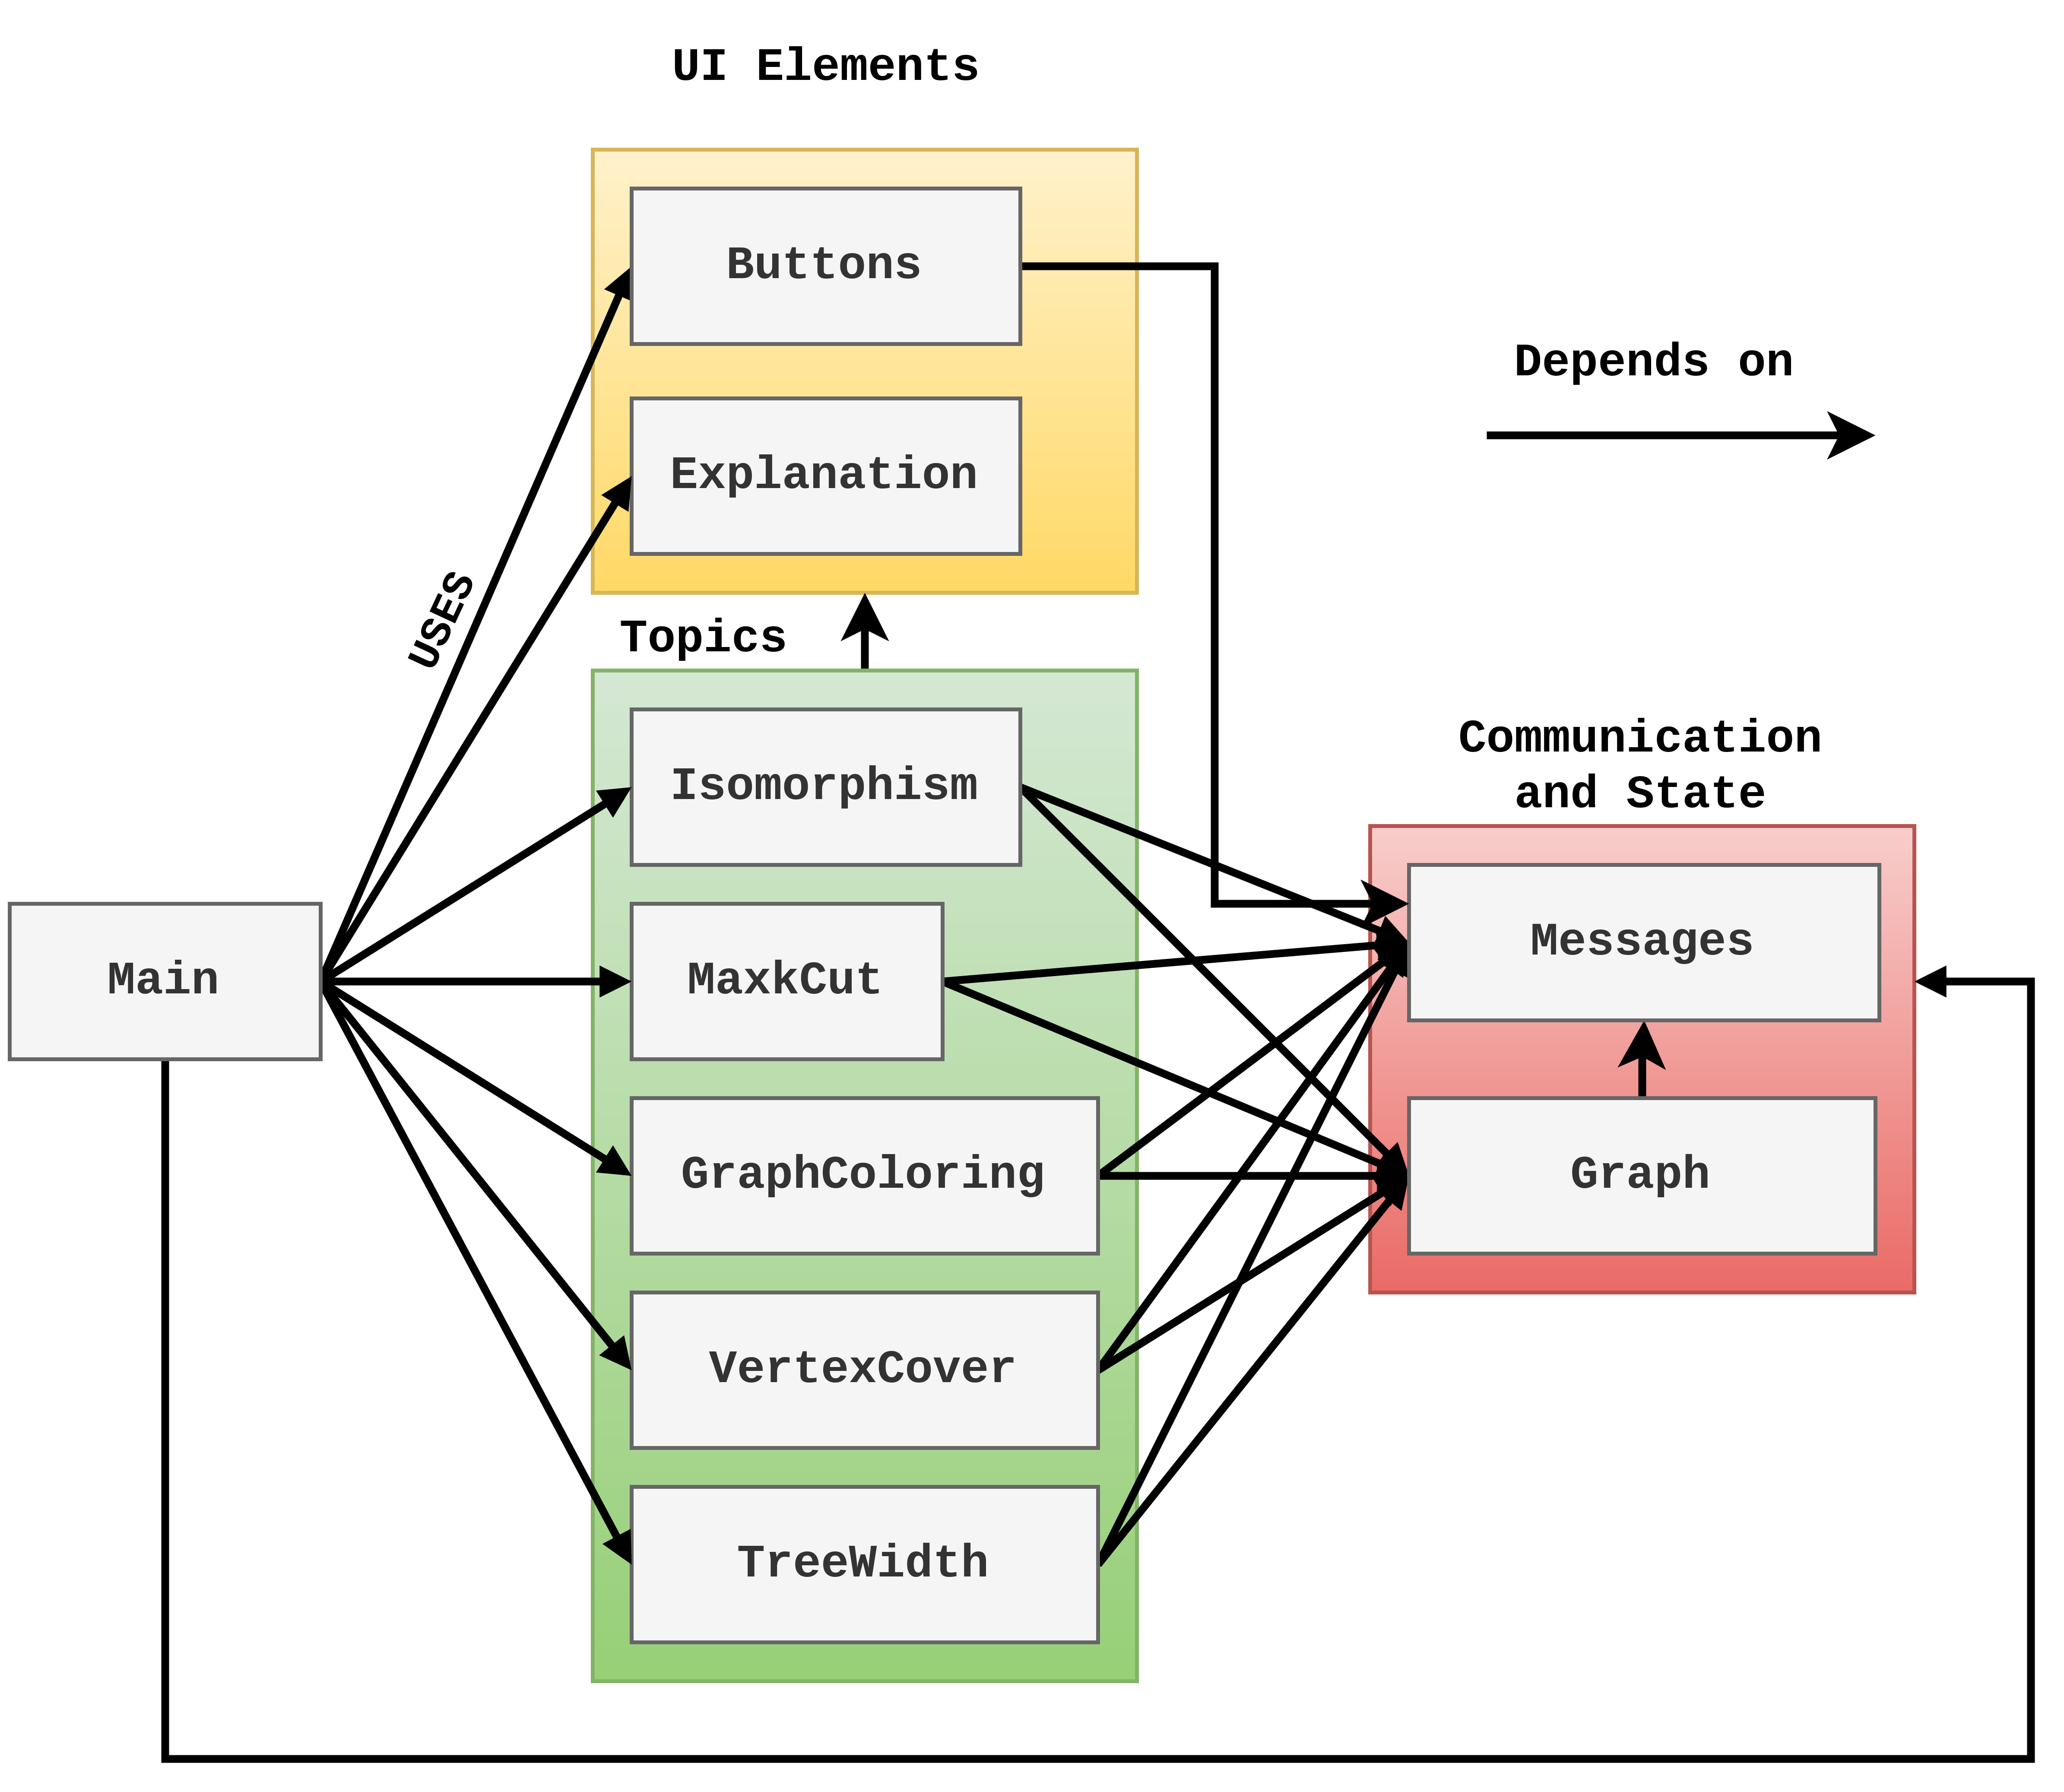
\includegraphics[width=3.22in]{Modules}
\caption{
        Modules in the Program. Arrows from the blunt end to the pointy end
        depict dependency. The main module contains the main logic of the application which
        uses different modules.  The most noteworthy of them are the modules
        related to the different graph theory topics.
        }
\end{figure}

\section{Software Engineering Practices}
In this section I will point out some of the software engineering practices that I used throughout the design and development of this application.

\subsection{Version Control}
The program along with the documentation and the dissertation report were
version controlled in a single GitHub repository. See \autoref{links:
repository}. A git repository gave me more confidence for undertaking risky and complex
refactoring and feature enhancement tasks by the way of creating separate branches
for all issues. A different branch was created for editing
documentation, and I made sure that modification in code files was not
done on this branch. Similarly, a branch for code refactoring did not modify the
documentation part hence separating concerns. Conveniently a branch could be
simply discarded if an adventure in a radical change in code went wrong.

\subsection{Continuous Deployment}
The web application concerning the project is deployed on the public Internet 
using Netlify. This service lets one host a front end website and is
connected to the master branch of the GitHub repository of the project. Every
time a new version is pushed to the master branch, the Netlify service fetches the new
version of the app from the repository, builds it according to the build script
present in the GitHub repository and deploys the web application on a specified
URL. The build and deployment can also be done manually by going to the
dashboard of the Netlify website. The build and deployment process primarily
consists of running a script to transpile Elm code to a JavaScript file and copy
the output along with the boiler plate HTML to the published directory.

If it is needed to deploy the application anew instantaneously (something which
is required to test the website for different screen sizes) a \emph{curl}
command with a specific \emph{build hook} URL is executed on the local
machine.  It triggers the deployment of the website from an up-to date copy of code in the master branch in the
repository.


\subsection{Documentation}
Documentation for the project was done in a continuous fashion in a variety of
ways, such as a wiki for code implementation and a guide for future work, time
logging for project management and report writing for the submission. 

The wiki was supported heavily from the code comments made to explain the
functions. Time logging brought a sense of discipline in the development efforts and
it also helped in estimating time required to complete the tasks which lay in
future and assess the learning curve.
